\documentclass[twoside]{book}

% Packages required by doxygen
\usepackage{fixltx2e}
\usepackage{calc}
\usepackage{doxygen}
\usepackage[export]{adjustbox} % also loads graphicx
\usepackage{graphicx}
\usepackage[utf8]{inputenc}
\usepackage{makeidx}
\usepackage{multicol}
\usepackage{multirow}
\PassOptionsToPackage{warn}{textcomp}
\usepackage{textcomp}
\usepackage[nointegrals]{wasysym}
\usepackage[table]{xcolor}

% Font selection
\usepackage[T1]{fontenc}
\usepackage[scaled=.90]{helvet}
\usepackage{courier}
\usepackage{amssymb}
\usepackage{sectsty}
\renewcommand{\familydefault}{\sfdefault}
\allsectionsfont{%
  \fontseries{bc}\selectfont%
  \color{darkgray}%
}
\renewcommand{\DoxyLabelFont}{%
  \fontseries{bc}\selectfont%
  \color{darkgray}%
}
\newcommand{\+}{\discretionary{\mbox{\scriptsize$\hookleftarrow$}}{}{}}

% Page & text layout
\usepackage{geometry}
\geometry{%
  a4paper,%
  top=2.5cm,%
  bottom=2.5cm,%
  left=2.5cm,%
  right=2.5cm%
}
\tolerance=750
\hfuzz=15pt
\hbadness=750
\setlength{\emergencystretch}{15pt}
\setlength{\parindent}{0cm}
\setlength{\parskip}{3ex plus 2ex minus 2ex}
\makeatletter
\renewcommand{\paragraph}{%
  \@startsection{paragraph}{4}{0ex}{-1.0ex}{1.0ex}{%
    \normalfont\normalsize\bfseries\SS@parafont%
  }%
}
\renewcommand{\subparagraph}{%
  \@startsection{subparagraph}{5}{0ex}{-1.0ex}{1.0ex}{%
    \normalfont\normalsize\bfseries\SS@subparafont%
  }%
}
\makeatother

% Headers & footers
\usepackage{fancyhdr}
\pagestyle{fancyplain}
\fancyhead[LE]{\fancyplain{}{\bfseries\thepage}}
\fancyhead[CE]{\fancyplain{}{}}
\fancyhead[RE]{\fancyplain{}{\bfseries\leftmark}}
\fancyhead[LO]{\fancyplain{}{\bfseries\rightmark}}
\fancyhead[CO]{\fancyplain{}{}}
\fancyhead[RO]{\fancyplain{}{\bfseries\thepage}}
\fancyfoot[LE]{\fancyplain{}{}}
\fancyfoot[CE]{\fancyplain{}{}}
\fancyfoot[RE]{\fancyplain{}{\bfseries\scriptsize Generated by Doxygen }}
\fancyfoot[LO]{\fancyplain{}{\bfseries\scriptsize Generated by Doxygen }}
\fancyfoot[CO]{\fancyplain{}{}}
\fancyfoot[RO]{\fancyplain{}{}}
\renewcommand{\footrulewidth}{0.4pt}
\renewcommand{\chaptermark}[1]{%
  \markboth{#1}{}%
}
\renewcommand{\sectionmark}[1]{%
  \markright{\thesection\ #1}%
}

% Indices & bibliography
\usepackage{natbib}
\usepackage[titles]{tocloft}
\setcounter{tocdepth}{3}
\setcounter{secnumdepth}{5}
\makeindex

% Packages requested by user
\usepackage{amsmath}

% Hyperlinks (required, but should be loaded last)
\usepackage{ifpdf}
\ifpdf
  \usepackage[pdftex,pagebackref=true]{hyperref}
\else
  \usepackage[ps2pdf,pagebackref=true]{hyperref}
\fi
\hypersetup{%
  colorlinks=true,%
  linkcolor=blue,%
  citecolor=blue,%
  unicode%
}

% Custom commands
\newcommand{\clearemptydoublepage}{%
  \newpage{\pagestyle{empty}\cleardoublepage}%
}

\usepackage{caption}
\captionsetup{labelsep=space,justification=centering,font={bf},singlelinecheck=off,skip=4pt,position=top}

%===== C O N T E N T S =====

\begin{document}

% Titlepage & ToC
\hypersetup{pageanchor=false,
             bookmarksnumbered=true,
             pdfencoding=unicode
            }
\pagenumbering{alph}
\begin{titlepage}
\vspace*{7cm}
\begin{center}%
{\Large S\+OM \\[1ex]\large 0.\+1.\+0 }\\
\vspace*{1cm}
{\large Generated by Doxygen 1.8.14}\\
\end{center}
\end{titlepage}
\clearemptydoublepage
\pagenumbering{roman}
\tableofcontents
\clearemptydoublepage
\pagenumbering{arabic}
\hypersetup{pageanchor=true}

%--- Begin generated contents ---
\chapter{Self\+Organizing\+Maps}
\label{md__r_e_a_d_m_e}
\Hypertarget{md__r_e_a_d_m_e}
Self organizing maps implementation. 
\chapter{Class Index}
\section{Class List}
Here are the classes, structs, unions and interfaces with brief descriptions\+:\begin{DoxyCompactList}
\item\contentsline{section}{\mbox{\hyperlink{class_s_o_m}{S\+O\+M$<$ T $>$}} \\*Self-\/\+Organizing Maps implementation. }{\pageref{class_s_o_m}}{}
\end{DoxyCompactList}

\chapter{File Index}
\section{File List}
Here is a list of all documented files with brief descriptions\+:\begin{DoxyCompactList}
\item\contentsline{section}{\mbox{\hyperlink{_s_o_m_8h}{S\+O\+M.\+h}} }{\pageref{_s_o_m_8h}}{}
\end{DoxyCompactList}

\chapter{Class Documentation}
\hypertarget{class_s_o_m}{}\section{S\+OM$<$ T $>$ Class Template Reference}
\label{class_s_o_m}\index{S\+O\+M$<$ T $>$@{S\+O\+M$<$ T $>$}}


Self-\/\+Organizing Maps implementation.  




{\ttfamily \#include $<$S\+O\+M.\+h$>$}

\subsection*{Public Member Functions}
\begin{DoxyCompactItemize}
\item 
\mbox{\hyperlink{class_s_o_m_ae68da19aade22031ef375a4cc6c6cec4}{S\+OM}} (int w, int h, int d)
\begin{DoxyCompactList}\small\item\em Overloaded Constructor. Weights are randomly assigned between \mbox{[}0,1). \end{DoxyCompactList}\item 
\mbox{\hyperlink{class_s_o_m_a980c547746b4458a6dfd9d60703bbf7d}{S\+OM}} (int w, int h, int d, \mbox{\hyperlink{_s_o_m_8h_a55f65662fc7b41a21c646e37b51ae9d9}{B\+M\+Dist\+Type}} \mbox{\hyperlink{class_s_o_m_a8d02f1179ca154170fd3bf349a112706}{bmdist\+Type}}, \mbox{\hyperlink{_s_o_m_8h_a69503914f8053c00b814b3096e784d72}{Distance\+Type}} \mbox{\hyperlink{class_s_o_m_a2cdff72776415d723fba0e90b7df5bc8}{distance\+Type}})
\begin{DoxyCompactList}\small\item\em Overloaded Constructor. Weights are randomly assigned between \mbox{[}0,1). \end{DoxyCompactList}\item 
void \mbox{\hyperlink{class_s_o_m_a9c93f45267b1653317a3ff60df207233}{train}} (const std\+::vector$<$ std\+::vector$<$ T $>$$>$ \&samples, unsigned int iterations, double s\+\_\+learn\+\_\+rate, double f\+\_\+learn\+\_\+rate, double neighborhood\+Size)
\begin{DoxyCompactList}\small\item\em trains the \mbox{\hyperlink{class_s_o_m}{S\+OM}}. If there are less samples than th \#N of iterations, then the samples are repeated cyclically. \end{DoxyCompactList}\item 
std\+::vector$<$ T $>$ \mbox{\hyperlink{class_s_o_m_ae6347cd92d0b112e940808480f718ea2}{cluster}} (const std\+::vector$<$ T $>$ \&sample)
\begin{DoxyCompactList}\small\item\em clusters the input sample. \end{DoxyCompactList}\item 
virtual \mbox{\hyperlink{class_s_o_m_ab81cf7a71cb418ff7c37b2e496253bb3}{$\sim$\+S\+OM}} ()
\begin{DoxyCompactList}\small\item\em Empty destructor. \end{DoxyCompactList}\item 
T $\ast$const \mbox{\hyperlink{class_s_o_m_a2d601f7afacfc9f7bd97d8725dd75f55}{node\+At}} (int i, int j) const
\begin{DoxyCompactList}\small\item\em get node (neuron) weights at given position. \end{DoxyCompactList}\item 
void \mbox{\hyperlink{class_s_o_m_a9db54f99d0beb0a96c97d9043032cb56}{set\+Node\+At}} (int i, int j, const std\+::vector$<$ T $>$ \&val)
\begin{DoxyCompactList}\small\item\em assign values to weights of the neuron at given indices. \end{DoxyCompactList}\item 
void \mbox{\hyperlink{class_s_o_m_a81e6d3a9b190872b8b8fd5bac513cf20}{load}} (const std\+::string \&model\+\_\+path, const \mbox{\hyperlink{_s_o_m_8h_a78e44725402091318ad38c42d5c34e69}{S\+O\+M\+File\+Format}} \&ff)
\begin{DoxyCompactList}\small\item\em loads the trained \mbox{\hyperlink{class_s_o_m}{S\+OM}} network from the file. \end{DoxyCompactList}\item 
void \mbox{\hyperlink{class_s_o_m_a3969de21028793245f1b5e88a040f6b5}{save}} (const std\+::string \&model\+\_\+path, const \mbox{\hyperlink{_s_o_m_8h_a78e44725402091318ad38c42d5c34e69}{S\+O\+M\+File\+Format}} \&ff)
\begin{DoxyCompactList}\small\item\em saves the trained \mbox{\hyperlink{class_s_o_m}{S\+OM}} to the file. \end{DoxyCompactList}\item 
int \mbox{\hyperlink{class_s_o_m_a47f9c6ce9c61975584806d75759a684b}{cols}} ()
\begin{DoxyCompactList}\small\item\em get \#N of columns (width) of \mbox{\hyperlink{class_s_o_m}{S\+OM}} lattice \end{DoxyCompactList}\item 
int \mbox{\hyperlink{class_s_o_m_ab56a48e18e8d571aa8f5f097810a20e8}{rows}} ()
\begin{DoxyCompactList}\small\item\em get \#N of rows (height) of \mbox{\hyperlink{class_s_o_m}{S\+OM}} lattice \end{DoxyCompactList}\item 
int \mbox{\hyperlink{class_s_o_m_a82010df22b8a692601621932f4d5a389}{dims}} ()
\begin{DoxyCompactList}\small\item\em get dimensions (codebook vector size) of \mbox{\hyperlink{class_s_o_m}{S\+OM}} \end{DoxyCompactList}\item 
T \mbox{\hyperlink{class_s_o_m_a1922509a8fecfd1598624c0348ac83c6}{calc\+Best\+Matching\+Unit}} (const std\+::vector$<$ T $>$ \&sample, int \&y, int \&x) const
\begin{DoxyCompactList}\small\item\em calculates Best Matching Unit (winning neuron). \end{DoxyCompactList}\end{DoxyCompactItemize}
\subsection*{Private Member Functions}
\begin{DoxyCompactItemize}
\item 
T \mbox{\hyperlink{class_s_o_m_a81a8ee36536002796b31d03f9a67ded1}{euclidean\+Distance}} (const std\+::vector$<$ T $>$ \&v1, const std\+::vector$<$ T $>$ \&v2) const
\begin{DoxyCompactList}\small\item\em calculates Euclidean Distance between 2 vectors. \end{DoxyCompactList}\item 
T \mbox{\hyperlink{class_s_o_m_ad57639354c1d0d50222691e05f328fb5}{squared\+Euclidean\+Distance}} (const std\+::vector$<$ T $>$ \&v1, const std\+::vector$<$ T $>$ \&v2) const
\begin{DoxyCompactList}\small\item\em calculates squared euclidean distance between 2 vectors. \end{DoxyCompactList}\item 
T \mbox{\hyperlink{class_s_o_m_a1cc6e3ecbbf41df75f3603fd0fa8fb86}{calc\+Gaussian}} (T mean, T std\+Dev, T x) const
\begin{DoxyCompactList}\small\item\em calculates Gaussian function of given x. \end{DoxyCompactList}\item 
T \mbox{\hyperlink{class_s_o_m_aa61653cc314a75b7315951c27ec2bc2a}{calc\+Gaussian2D}} (T meanX, T meanY, T sigmaX, T sigmaY, T x, T y) const
\begin{DoxyCompactList}\small\item\em calculates 2D Gaussian function of given input pair (x,y). \end{DoxyCompactList}\item 
T \mbox{\hyperlink{class_s_o_m_a3a34e3e6e83577c1afa7b27dee2ab544}{calc\+Gaussian2D}} (int meanX, int meanY, T sigma, int x, int y) const
\begin{DoxyCompactList}\small\item\em calculates 2D Gaussian function of given input pair (x,y). This method uses the same sigma for X and Y dimensions. \end{DoxyCompactList}\item 
T \mbox{\hyperlink{class_s_o_m_a1bdfadf3e4dbd2a9cb229e72cf52fb0b}{euclidean\+Distance}} (const std\+::vector$<$ T $>$ \&v1, const T $\ast$v2) const
\begin{DoxyCompactList}\small\item\em calculates Euclidean Distance between 2 vectors. This method overloads () as second parameter is pointer to T for performance reasons. \end{DoxyCompactList}\item 
T \mbox{\hyperlink{class_s_o_m_aae16d4dfa51332b631c314dc82ef9145}{dot\+Product}} (const std\+::vector$<$ T $>$ \&v1, const T $\ast$v2) const
\begin{DoxyCompactList}\small\item\em calculates Dot Product of 2 vectors. \end{DoxyCompactList}\item 
T \mbox{\hyperlink{class_s_o_m_a577f703f087e87c5d8580665540a9833}{cosine\+Similarity}} (const std\+::vector$<$ T $>$ \&v1, const T $\ast$v2) const
\begin{DoxyCompactList}\small\item\em calculates cosine similarity of 2 vectors. \end{DoxyCompactList}\item 
T \mbox{\hyperlink{class_s_o_m_a9dbf0a67e0afcc612ff68a7f287c8450}{L2norm}} (const std\+::vector$<$ T $>$ \&v1)
\begin{DoxyCompactList}\small\item\em calculates L2 norm of a vector \end{DoxyCompactList}\end{DoxyCompactItemize}
\subsection*{Private Attributes}
\begin{DoxyCompactItemize}
\item 
\mbox{\hyperlink{_s_o_m_8h_a55f65662fc7b41a21c646e37b51ae9d9}{B\+M\+Dist\+Type}} \mbox{\hyperlink{class_s_o_m_a8d02f1179ca154170fd3bf349a112706}{bmdist\+Type}}
\begin{DoxyCompactList}\small\item\em Best Matching Unit neighbour distance update type of the \mbox{\hyperlink{class_s_o_m}{S\+OM}}. \end{DoxyCompactList}\item 
\mbox{\hyperlink{_s_o_m_8h_a69503914f8053c00b814b3096e784d72}{Distance\+Type}} \mbox{\hyperlink{class_s_o_m_a2cdff72776415d723fba0e90b7df5bc8}{distance\+Type}}
\begin{DoxyCompactList}\small\item\em distance metric that is used when B\+MU is calculated see () \end{DoxyCompactList}\item 
int \mbox{\hyperlink{class_s_o_m_a99414c651f0e1371d0e16437a1769fd9}{W}}
\begin{DoxyCompactList}\small\item\em grid width \end{DoxyCompactList}\item 
int \mbox{\hyperlink{class_s_o_m_a34ef6069c3f522ece1b0dad99484a9c3}{H}}
\begin{DoxyCompactList}\small\item\em grid height \end{DoxyCompactList}\item 
int \mbox{\hyperlink{class_s_o_m_a125c2393ee9e0f75a42bd03db31a2f15}{D}}
\begin{DoxyCompactList}\small\item\em size of the weight vector of the each node. \end{DoxyCompactList}\item 
std\+::vector$<$ T $>$ \mbox{\hyperlink{class_s_o_m_abb0a6072eb9fd4c3bd297814e654f561}{weights}}
\begin{DoxyCompactList}\small\item\em weights / nodes of \mbox{\hyperlink{class_s_o_m}{S\+OM}} \end{DoxyCompactList}\end{DoxyCompactItemize}
\subsection*{Friends}
\begin{DoxyCompactItemize}
\item 
\mbox{\Hypertarget{class_s_o_m_a16061bd717ac865e42d9fb288945b81a}\label{class_s_o_m_a16061bd717ac865e42d9fb288945b81a}} 
Y\+A\+M\+L\+::\+Emitter \& {\bfseries operator$<$$<$} (Y\+A\+M\+L\+::\+Emitter \&out, const \mbox{\hyperlink{class_s_o_m}{S\+OM}}$<$ T $>$ \&som)
\item 
\mbox{\Hypertarget{class_s_o_m_adf2105b08320a0f005bbe1b55c91712a}\label{class_s_o_m_adf2105b08320a0f005bbe1b55c91712a}} 
void {\bfseries operator$>$$>$} (const Y\+A\+M\+L\+::\+Node \&node, \mbox{\hyperlink{class_s_o_m}{S\+OM}}$<$ T $>$ \&som)
\end{DoxyCompactItemize}


\subsection{Detailed Description}
\subsubsection*{template$<$class T$>$\newline
class S\+O\+M$<$ T $>$}

Self-\/\+Organizing Maps implementation. 



\subsection{Constructor \& Destructor Documentation}
\mbox{\Hypertarget{class_s_o_m_ae68da19aade22031ef375a4cc6c6cec4}\label{class_s_o_m_ae68da19aade22031ef375a4cc6c6cec4}} 
\index{S\+OM@{S\+OM}!S\+OM@{S\+OM}}
\index{S\+OM@{S\+OM}!S\+OM@{S\+OM}}
\subsubsection{\texorpdfstring{S\+O\+M()}{SOM()}\hspace{0.1cm}{\footnotesize\ttfamily [1/2]}}
{\footnotesize\ttfamily template$<$class T$>$ \\
\mbox{\hyperlink{class_s_o_m}{S\+OM}}$<$ T $>$\+::\mbox{\hyperlink{class_s_o_m}{S\+OM}} (\begin{DoxyParamCaption}\item[{int}]{w,  }\item[{int}]{h,  }\item[{int}]{d }\end{DoxyParamCaption})\hspace{0.3cm}{\ttfamily [inline]}}



Overloaded Constructor. Weights are randomly assigned between \mbox{[}0,1). 


\begin{DoxyParams}{Parameters}
{\em w} & width\\
\hline
{\em h} & height\\
\hline
{\em d} & \#N of dimensions (codebook size).\\
\hline
\end{DoxyParams}
\mbox{\Hypertarget{class_s_o_m_a980c547746b4458a6dfd9d60703bbf7d}\label{class_s_o_m_a980c547746b4458a6dfd9d60703bbf7d}} 
\index{S\+OM@{S\+OM}!S\+OM@{S\+OM}}
\index{S\+OM@{S\+OM}!S\+OM@{S\+OM}}
\subsubsection{\texorpdfstring{S\+O\+M()}{SOM()}\hspace{0.1cm}{\footnotesize\ttfamily [2/2]}}
{\footnotesize\ttfamily template$<$class T$>$ \\
\mbox{\hyperlink{class_s_o_m}{S\+OM}}$<$ T $>$\+::\mbox{\hyperlink{class_s_o_m}{S\+OM}} (\begin{DoxyParamCaption}\item[{int}]{w,  }\item[{int}]{h,  }\item[{int}]{d,  }\item[{\mbox{\hyperlink{_s_o_m_8h_a55f65662fc7b41a21c646e37b51ae9d9}{B\+M\+Dist\+Type}}}]{bmdist\+Type,  }\item[{\mbox{\hyperlink{_s_o_m_8h_a69503914f8053c00b814b3096e784d72}{Distance\+Type}}}]{distance\+Type }\end{DoxyParamCaption})\hspace{0.3cm}{\ttfamily [inline]}}



Overloaded Constructor. Weights are randomly assigned between \mbox{[}0,1). 


\begin{DoxyParams}{Parameters}
{\em w} & Width.\\
\hline
{\em h} & Height.\\
\hline
{\em d} & \#N of Dimensions.\\
\hline
{\em bmdist\+Type} & B\+MU update coefficients type. \\
\hline
{\em distance\+Type} & Distance metric type to use. \\
\hline
\end{DoxyParams}
\mbox{\Hypertarget{class_s_o_m_ab81cf7a71cb418ff7c37b2e496253bb3}\label{class_s_o_m_ab81cf7a71cb418ff7c37b2e496253bb3}} 
\index{S\+OM@{S\+OM}!````~S\+OM@{$\sim$\+S\+OM}}
\index{````~S\+OM@{$\sim$\+S\+OM}!S\+OM@{S\+OM}}
\subsubsection{\texorpdfstring{$\sim$\+S\+O\+M()}{~SOM()}}
{\footnotesize\ttfamily template$<$class T$>$ \\
virtual \mbox{\hyperlink{class_s_o_m}{S\+OM}}$<$ T $>$\+::$\sim$\mbox{\hyperlink{class_s_o_m}{S\+OM}} (\begin{DoxyParamCaption}{ }\end{DoxyParamCaption})\hspace{0.3cm}{\ttfamily [inline]}, {\ttfamily [virtual]}}



Empty destructor. 



\subsection{Member Function Documentation}
\mbox{\Hypertarget{class_s_o_m_a1922509a8fecfd1598624c0348ac83c6}\label{class_s_o_m_a1922509a8fecfd1598624c0348ac83c6}} 
\index{S\+OM@{S\+OM}!calc\+Best\+Matching\+Unit@{calc\+Best\+Matching\+Unit}}
\index{calc\+Best\+Matching\+Unit@{calc\+Best\+Matching\+Unit}!S\+OM@{S\+OM}}
\subsubsection{\texorpdfstring{calc\+Best\+Matching\+Unit()}{calcBestMatchingUnit()}}
{\footnotesize\ttfamily template$<$class T$>$ \\
T \mbox{\hyperlink{class_s_o_m}{S\+OM}}$<$ T $>$\+::calc\+Best\+Matching\+Unit (\begin{DoxyParamCaption}\item[{const std\+::vector$<$ T $>$ \&}]{sample,  }\item[{int \&}]{y,  }\item[{int \&}]{x }\end{DoxyParamCaption}) const\hspace{0.3cm}{\ttfamily [inline]}}



calculates Best Matching Unit (winning neuron). 


\begin{DoxyParams}{Parameters}
{\em sample} & input sample\\
\hline
{\em y} & index of the 0th dimension (rows) of the winning neuron \\
\hline
{\em x} & index of the 1th dimension (columns) of the winning neuron \\
\hline
\end{DoxyParams}
\begin{DoxyReturn}{Returns}
distance between B\+MU and sample 
\end{DoxyReturn}
\mbox{\Hypertarget{class_s_o_m_a1cc6e3ecbbf41df75f3603fd0fa8fb86}\label{class_s_o_m_a1cc6e3ecbbf41df75f3603fd0fa8fb86}} 
\index{S\+OM@{S\+OM}!calc\+Gaussian@{calc\+Gaussian}}
\index{calc\+Gaussian@{calc\+Gaussian}!S\+OM@{S\+OM}}
\subsubsection{\texorpdfstring{calc\+Gaussian()}{calcGaussian()}}
{\footnotesize\ttfamily template$<$class T$>$ \\
T \mbox{\hyperlink{class_s_o_m}{S\+OM}}$<$ T $>$\+::calc\+Gaussian (\begin{DoxyParamCaption}\item[{T}]{mean,  }\item[{T}]{std\+Dev,  }\item[{T}]{x }\end{DoxyParamCaption}) const\hspace{0.3cm}{\ttfamily [inline]}, {\ttfamily [private]}}



calculates Gaussian function of given x. 

$ f(x)=\frac{1}{(\sigma \sqrt{(2\pi)}}e^{(\frac{-(x-\mu)^2}{2\sigma^2})} $ 


\begin{DoxyParams}{Parameters}
{\em mean} & mean of the Gaussian distribution\\
\hline
{\em std\+Dev} & standarad deviation\\
\hline
{\em x} & input value\\
\hline
\end{DoxyParams}
\begin{DoxyReturn}{Returns}
Gaussian function of the given x.
\end{DoxyReturn}
\mbox{\Hypertarget{class_s_o_m_aa61653cc314a75b7315951c27ec2bc2a}\label{class_s_o_m_aa61653cc314a75b7315951c27ec2bc2a}} 
\index{S\+OM@{S\+OM}!calc\+Gaussian2D@{calc\+Gaussian2D}}
\index{calc\+Gaussian2D@{calc\+Gaussian2D}!S\+OM@{S\+OM}}
\subsubsection{\texorpdfstring{calc\+Gaussian2\+D()}{calcGaussian2D()}\hspace{0.1cm}{\footnotesize\ttfamily [1/2]}}
{\footnotesize\ttfamily template$<$class T$>$ \\
T \mbox{\hyperlink{class_s_o_m}{S\+OM}}$<$ T $>$\+::calc\+Gaussian2D (\begin{DoxyParamCaption}\item[{T}]{meanX,  }\item[{T}]{meanY,  }\item[{T}]{sigmaX,  }\item[{T}]{sigmaY,  }\item[{T}]{x,  }\item[{T}]{y }\end{DoxyParamCaption}) const\hspace{0.3cm}{\ttfamily [inline]}, {\ttfamily [private]}}



calculates 2D Gaussian function of given input pair (x,y). 

$ f(x,y)=\frac{1}{(2\pi\sigma_x\sigma_y)}e^{(-[(x-\mu_x)^2/(2\sigma_x^2)+(y-\mu_y)^2 /(2\sigma_y^2)])} $ . 


\begin{DoxyParams}{Parameters}
{\em meanX} & mean value in X dimension. \\
\hline
{\em meanY} & mean value in Y dimension. \\
\hline
{\em sigmaX} & standarad deviation in X dimension. \\
\hline
{\em sigmaY} & standarad deviation in Y dimension. \\
\hline
{\em x} & input value (X dimension). \\
\hline
{\em y} & input value (Y dimension). \\
\hline
\end{DoxyParams}
\begin{DoxyReturn}{Returns}
2d gaussian function value of the given (x,y) pair.
\end{DoxyReturn}
\mbox{\Hypertarget{class_s_o_m_a3a34e3e6e83577c1afa7b27dee2ab544}\label{class_s_o_m_a3a34e3e6e83577c1afa7b27dee2ab544}} 
\index{S\+OM@{S\+OM}!calc\+Gaussian2D@{calc\+Gaussian2D}}
\index{calc\+Gaussian2D@{calc\+Gaussian2D}!S\+OM@{S\+OM}}
\subsubsection{\texorpdfstring{calc\+Gaussian2\+D()}{calcGaussian2D()}\hspace{0.1cm}{\footnotesize\ttfamily [2/2]}}
{\footnotesize\ttfamily template$<$class T$>$ \\
T \mbox{\hyperlink{class_s_o_m}{S\+OM}}$<$ T $>$\+::calc\+Gaussian2D (\begin{DoxyParamCaption}\item[{int}]{meanX,  }\item[{int}]{meanY,  }\item[{T}]{sigma,  }\item[{int}]{x,  }\item[{int}]{y }\end{DoxyParamCaption}) const\hspace{0.3cm}{\ttfamily [inline]}, {\ttfamily [private]}}



calculates 2D Gaussian function of given input pair (x,y). This method uses the same sigma for X and Y dimensions. 

$ f(x,y)=\frac{1}{(2\pi\sigma^2)}e^{(-[(x-\mu_x)^2+(y-\mu_y)^2]/(2\sigma^2))} $. 


\begin{DoxyParams}{Parameters}
{\em meanX} & mean value in X dimension.\\
\hline
{\em meanY} & mean value in Y dimension.\\
\hline
{\em sigma} & standarad deviation (sigma\+Vector=\mbox{[}sigma, sigma\mbox{]})\\
\hline
{\em x} & input value (X dimension).\\
\hline
{\em y} & input value (Y dimension).\\
\hline
\end{DoxyParams}
\begin{DoxyReturn}{Returns}
2d gaussian function value of the given (x,y) pair.
\end{DoxyReturn}
\mbox{\Hypertarget{class_s_o_m_ae6347cd92d0b112e940808480f718ea2}\label{class_s_o_m_ae6347cd92d0b112e940808480f718ea2}} 
\index{S\+OM@{S\+OM}!cluster@{cluster}}
\index{cluster@{cluster}!S\+OM@{S\+OM}}
\subsubsection{\texorpdfstring{cluster()}{cluster()}}
{\footnotesize\ttfamily template$<$class T$>$ \\
std\+::vector$<$T$>$ \mbox{\hyperlink{class_s_o_m}{S\+OM}}$<$ T $>$\+::cluster (\begin{DoxyParamCaption}\item[{const std\+::vector$<$ T $>$ \&}]{sample }\end{DoxyParamCaption})\hspace{0.3cm}{\ttfamily [inline]}}



clusters the input sample. 


\begin{DoxyParams}{Parameters}
{\em sample} & input sample\\
\hline
\end{DoxyParams}
\begin{DoxyReturn}{Returns}
Winner neuron\textquotesingle{}s weight vector, which corresponds to the most similar weights to input pattern. 
\end{DoxyReturn}
\mbox{\Hypertarget{class_s_o_m_a47f9c6ce9c61975584806d75759a684b}\label{class_s_o_m_a47f9c6ce9c61975584806d75759a684b}} 
\index{S\+OM@{S\+OM}!cols@{cols}}
\index{cols@{cols}!S\+OM@{S\+OM}}
\subsubsection{\texorpdfstring{cols()}{cols()}}
{\footnotesize\ttfamily template$<$class T$>$ \\
int \mbox{\hyperlink{class_s_o_m}{S\+OM}}$<$ T $>$\+::cols (\begin{DoxyParamCaption}{ }\end{DoxyParamCaption})\hspace{0.3cm}{\ttfamily [inline]}}



get \#N of columns (width) of \mbox{\hyperlink{class_s_o_m}{S\+OM}} lattice 

\begin{DoxyReturn}{Returns}

\end{DoxyReturn}
\mbox{\Hypertarget{class_s_o_m_a577f703f087e87c5d8580665540a9833}\label{class_s_o_m_a577f703f087e87c5d8580665540a9833}} 
\index{S\+OM@{S\+OM}!cosine\+Similarity@{cosine\+Similarity}}
\index{cosine\+Similarity@{cosine\+Similarity}!S\+OM@{S\+OM}}
\subsubsection{\texorpdfstring{cosine\+Similarity()}{cosineSimilarity()}}
{\footnotesize\ttfamily template$<$class T$>$ \\
T \mbox{\hyperlink{class_s_o_m}{S\+OM}}$<$ T $>$\+::cosine\+Similarity (\begin{DoxyParamCaption}\item[{const std\+::vector$<$ T $>$ \&}]{v1,  }\item[{const T $\ast$}]{v2 }\end{DoxyParamCaption}) const\hspace{0.3cm}{\ttfamily [inline]}, {\ttfamily [private]}}



calculates cosine similarity of 2 vectors. 


\begin{DoxyParams}{Parameters}
{\em v1} & vector 1\\
\hline
{\em v2} & vector 2\\
\hline
\end{DoxyParams}
\begin{DoxyReturn}{Returns}
resulting scalar value of cosine similarity
\end{DoxyReturn}
\mbox{\Hypertarget{class_s_o_m_a82010df22b8a692601621932f4d5a389}\label{class_s_o_m_a82010df22b8a692601621932f4d5a389}} 
\index{S\+OM@{S\+OM}!dims@{dims}}
\index{dims@{dims}!S\+OM@{S\+OM}}
\subsubsection{\texorpdfstring{dims()}{dims()}}
{\footnotesize\ttfamily template$<$class T$>$ \\
int \mbox{\hyperlink{class_s_o_m}{S\+OM}}$<$ T $>$\+::dims (\begin{DoxyParamCaption}{ }\end{DoxyParamCaption})\hspace{0.3cm}{\ttfamily [inline]}}



get dimensions (codebook vector size) of \mbox{\hyperlink{class_s_o_m}{S\+OM}} 

\begin{DoxyReturn}{Returns}

\end{DoxyReturn}
\mbox{\Hypertarget{class_s_o_m_aae16d4dfa51332b631c314dc82ef9145}\label{class_s_o_m_aae16d4dfa51332b631c314dc82ef9145}} 
\index{S\+OM@{S\+OM}!dot\+Product@{dot\+Product}}
\index{dot\+Product@{dot\+Product}!S\+OM@{S\+OM}}
\subsubsection{\texorpdfstring{dot\+Product()}{dotProduct()}}
{\footnotesize\ttfamily template$<$class T$>$ \\
T \mbox{\hyperlink{class_s_o_m}{S\+OM}}$<$ T $>$\+::dot\+Product (\begin{DoxyParamCaption}\item[{const std\+::vector$<$ T $>$ \&}]{v1,  }\item[{const T $\ast$}]{v2 }\end{DoxyParamCaption}) const\hspace{0.3cm}{\ttfamily [inline]}, {\ttfamily [private]}}



calculates Dot Product of 2 vectors. 


\begin{DoxyParams}{Parameters}
{\em v1} & vector 1\\
\hline
{\em v2} & vector 2\\
\hline
\end{DoxyParams}
\begin{DoxyReturn}{Returns}
resulting scalar value of dot product 
\end{DoxyReturn}
\mbox{\Hypertarget{class_s_o_m_a81a8ee36536002796b31d03f9a67ded1}\label{class_s_o_m_a81a8ee36536002796b31d03f9a67ded1}} 
\index{S\+OM@{S\+OM}!euclidean\+Distance@{euclidean\+Distance}}
\index{euclidean\+Distance@{euclidean\+Distance}!S\+OM@{S\+OM}}
\subsubsection{\texorpdfstring{euclidean\+Distance()}{euclideanDistance()}\hspace{0.1cm}{\footnotesize\ttfamily [1/2]}}
{\footnotesize\ttfamily template$<$class T$>$ \\
T \mbox{\hyperlink{class_s_o_m}{S\+OM}}$<$ T $>$\+::euclidean\+Distance (\begin{DoxyParamCaption}\item[{const std\+::vector$<$ T $>$ \&}]{v1,  }\item[{const std\+::vector$<$ T $>$ \&}]{v2 }\end{DoxyParamCaption}) const\hspace{0.3cm}{\ttfamily [inline]}, {\ttfamily [private]}}



calculates Euclidean Distance between 2 vectors. 


\begin{DoxyParams}{Parameters}
{\em v1} & vector 1\\
\hline
{\em v2} & vector 2\\
\hline
\end{DoxyParams}
\begin{DoxyReturn}{Returns}
euclidean distance
\end{DoxyReturn}
\mbox{\Hypertarget{class_s_o_m_a1bdfadf3e4dbd2a9cb229e72cf52fb0b}\label{class_s_o_m_a1bdfadf3e4dbd2a9cb229e72cf52fb0b}} 
\index{S\+OM@{S\+OM}!euclidean\+Distance@{euclidean\+Distance}}
\index{euclidean\+Distance@{euclidean\+Distance}!S\+OM@{S\+OM}}
\subsubsection{\texorpdfstring{euclidean\+Distance()}{euclideanDistance()}\hspace{0.1cm}{\footnotesize\ttfamily [2/2]}}
{\footnotesize\ttfamily template$<$class T$>$ \\
T \mbox{\hyperlink{class_s_o_m}{S\+OM}}$<$ T $>$\+::euclidean\+Distance (\begin{DoxyParamCaption}\item[{const std\+::vector$<$ T $>$ \&}]{v1,  }\item[{const T $\ast$}]{v2 }\end{DoxyParamCaption}) const\hspace{0.3cm}{\ttfamily [inline]}, {\ttfamily [private]}}



calculates Euclidean Distance between 2 vectors. This method overloads () as second parameter is pointer to T for performance reasons. 


\begin{DoxyParams}{Parameters}
{\em v1} & vector 1\\
\hline
{\em v2} & vector 2\\
\hline
\end{DoxyParams}
\begin{DoxyReturn}{Returns}
euclidean distance
\end{DoxyReturn}
\mbox{\Hypertarget{class_s_o_m_a9dbf0a67e0afcc612ff68a7f287c8450}\label{class_s_o_m_a9dbf0a67e0afcc612ff68a7f287c8450}} 
\index{S\+OM@{S\+OM}!L2norm@{L2norm}}
\index{L2norm@{L2norm}!S\+OM@{S\+OM}}
\subsubsection{\texorpdfstring{L2norm()}{L2norm()}}
{\footnotesize\ttfamily template$<$class T$>$ \\
T \mbox{\hyperlink{class_s_o_m}{S\+OM}}$<$ T $>$\+::L2norm (\begin{DoxyParamCaption}\item[{const std\+::vector$<$ T $>$ \&}]{v1 }\end{DoxyParamCaption})\hspace{0.3cm}{\ttfamily [inline]}, {\ttfamily [private]}}



calculates L2 norm of a vector 


\begin{DoxyParams}{Parameters}
{\em v1} & input vector\\
\hline
\end{DoxyParams}
\begin{DoxyReturn}{Returns}
scalar value of L2 norm.
\end{DoxyReturn}
\mbox{\Hypertarget{class_s_o_m_a81e6d3a9b190872b8b8fd5bac513cf20}\label{class_s_o_m_a81e6d3a9b190872b8b8fd5bac513cf20}} 
\index{S\+OM@{S\+OM}!load@{load}}
\index{load@{load}!S\+OM@{S\+OM}}
\subsubsection{\texorpdfstring{load()}{load()}}
{\footnotesize\ttfamily template$<$class T$>$ \\
void \mbox{\hyperlink{class_s_o_m}{S\+OM}}$<$ T $>$\+::load (\begin{DoxyParamCaption}\item[{const std\+::string \&}]{model\+\_\+path,  }\item[{const \mbox{\hyperlink{_s_o_m_8h_a78e44725402091318ad38c42d5c34e69}{S\+O\+M\+File\+Format}} \&}]{ff }\end{DoxyParamCaption})\hspace{0.3cm}{\ttfamily [inline]}}



loads the trained \mbox{\hyperlink{class_s_o_m}{S\+OM}} network from the file. 


\begin{DoxyParams}{Parameters}
{\em model\+\_\+path} & model path\\
\hline
\end{DoxyParams}
/// 
\begin{DoxyParams}{Parameters}
{\em ff} & file format\\
\hline
\end{DoxyParams}
\mbox{\Hypertarget{class_s_o_m_a2d601f7afacfc9f7bd97d8725dd75f55}\label{class_s_o_m_a2d601f7afacfc9f7bd97d8725dd75f55}} 
\index{S\+OM@{S\+OM}!node\+At@{node\+At}}
\index{node\+At@{node\+At}!S\+OM@{S\+OM}}
\subsubsection{\texorpdfstring{node\+At()}{nodeAt()}}
{\footnotesize\ttfamily template$<$class T$>$ \\
T$\ast$ const \mbox{\hyperlink{class_s_o_m}{S\+OM}}$<$ T $>$\+::node\+At (\begin{DoxyParamCaption}\item[{int}]{i,  }\item[{int}]{j }\end{DoxyParamCaption}) const\hspace{0.3cm}{\ttfamily [inline]}}



get node (neuron) weights at given position. 


\begin{DoxyParams}{Parameters}
{\em i} & index of the first dimension (rows) of the \mbox{\hyperlink{class_s_o_m}{S\+OM}} lattice. \\
\hline
{\em j} & index of the second dimension (columns) of the \mbox{\hyperlink{class_s_o_m}{S\+OM}} lattice.\\
\hline
\end{DoxyParams}
\begin{DoxyReturn}{Returns}
returns the pointer to Type T, which is the first element in the weight (codebook) vector of the corresponding \mbox{\hyperlink{class_s_o_m}{S\+OM}} node.
\end{DoxyReturn}
\mbox{\Hypertarget{class_s_o_m_ab56a48e18e8d571aa8f5f097810a20e8}\label{class_s_o_m_ab56a48e18e8d571aa8f5f097810a20e8}} 
\index{S\+OM@{S\+OM}!rows@{rows}}
\index{rows@{rows}!S\+OM@{S\+OM}}
\subsubsection{\texorpdfstring{rows()}{rows()}}
{\footnotesize\ttfamily template$<$class T$>$ \\
int \mbox{\hyperlink{class_s_o_m}{S\+OM}}$<$ T $>$\+::rows (\begin{DoxyParamCaption}{ }\end{DoxyParamCaption})\hspace{0.3cm}{\ttfamily [inline]}}



get \#N of rows (height) of \mbox{\hyperlink{class_s_o_m}{S\+OM}} lattice 

\begin{DoxyReturn}{Returns}

\end{DoxyReturn}
\mbox{\Hypertarget{class_s_o_m_a3969de21028793245f1b5e88a040f6b5}\label{class_s_o_m_a3969de21028793245f1b5e88a040f6b5}} 
\index{S\+OM@{S\+OM}!save@{save}}
\index{save@{save}!S\+OM@{S\+OM}}
\subsubsection{\texorpdfstring{save()}{save()}}
{\footnotesize\ttfamily template$<$class T$>$ \\
void \mbox{\hyperlink{class_s_o_m}{S\+OM}}$<$ T $>$\+::save (\begin{DoxyParamCaption}\item[{const std\+::string \&}]{model\+\_\+path,  }\item[{const \mbox{\hyperlink{_s_o_m_8h_a78e44725402091318ad38c42d5c34e69}{S\+O\+M\+File\+Format}} \&}]{ff }\end{DoxyParamCaption})\hspace{0.3cm}{\ttfamily [inline]}}



saves the trained \mbox{\hyperlink{class_s_o_m}{S\+OM}} to the file. 


\begin{DoxyParams}{Parameters}
{\em model\+\_\+path} & model file path\\
\hline
{\em ff} & file format\\
\hline
\end{DoxyParams}
\mbox{\Hypertarget{class_s_o_m_a9db54f99d0beb0a96c97d9043032cb56}\label{class_s_o_m_a9db54f99d0beb0a96c97d9043032cb56}} 
\index{S\+OM@{S\+OM}!set\+Node\+At@{set\+Node\+At}}
\index{set\+Node\+At@{set\+Node\+At}!S\+OM@{S\+OM}}
\subsubsection{\texorpdfstring{set\+Node\+At()}{setNodeAt()}}
{\footnotesize\ttfamily template$<$class T$>$ \\
void \mbox{\hyperlink{class_s_o_m}{S\+OM}}$<$ T $>$\+::set\+Node\+At (\begin{DoxyParamCaption}\item[{int}]{i,  }\item[{int}]{j,  }\item[{const std\+::vector$<$ T $>$ \&}]{val }\end{DoxyParamCaption})\hspace{0.3cm}{\ttfamily [inline]}}



assign values to weights of the neuron at given indices. 


\begin{DoxyParams}{Parameters}
{\em i} & index at 0th dimension (rows)\\
\hline
{\em j} & index at 1th dimension (columns)\\
\hline
{\em val} & value to set.\\
\hline
\end{DoxyParams}
\mbox{\Hypertarget{class_s_o_m_ad57639354c1d0d50222691e05f328fb5}\label{class_s_o_m_ad57639354c1d0d50222691e05f328fb5}} 
\index{S\+OM@{S\+OM}!squared\+Euclidean\+Distance@{squared\+Euclidean\+Distance}}
\index{squared\+Euclidean\+Distance@{squared\+Euclidean\+Distance}!S\+OM@{S\+OM}}
\subsubsection{\texorpdfstring{squared\+Euclidean\+Distance()}{squaredEuclideanDistance()}}
{\footnotesize\ttfamily template$<$class T$>$ \\
T \mbox{\hyperlink{class_s_o_m}{S\+OM}}$<$ T $>$\+::squared\+Euclidean\+Distance (\begin{DoxyParamCaption}\item[{const std\+::vector$<$ T $>$ \&}]{v1,  }\item[{const std\+::vector$<$ T $>$ \&}]{v2 }\end{DoxyParamCaption}) const\hspace{0.3cm}{\ttfamily [inline]}, {\ttfamily [private]}}



calculates squared euclidean distance between 2 vectors. 


\begin{DoxyParams}{Parameters}
{\em v1} & vector 1\\
\hline
{\em v2} & vector 2\\
\hline
\end{DoxyParams}
\begin{DoxyReturn}{Returns}
euclidean distance
\end{DoxyReturn}
\mbox{\Hypertarget{class_s_o_m_a9c93f45267b1653317a3ff60df207233}\label{class_s_o_m_a9c93f45267b1653317a3ff60df207233}} 
\index{S\+OM@{S\+OM}!train@{train}}
\index{train@{train}!S\+OM@{S\+OM}}
\subsubsection{\texorpdfstring{train()}{train()}}
{\footnotesize\ttfamily template$<$class T$>$ \\
void \mbox{\hyperlink{class_s_o_m}{S\+OM}}$<$ T $>$\+::train (\begin{DoxyParamCaption}\item[{const std\+::vector$<$ std\+::vector$<$ T $>$$>$ \&}]{samples,  }\item[{unsigned int}]{iterations,  }\item[{double}]{s\+\_\+learn\+\_\+rate,  }\item[{double}]{f\+\_\+learn\+\_\+rate,  }\item[{double}]{neighborhood\+Size }\end{DoxyParamCaption})\hspace{0.3cm}{\ttfamily [inline]}}



trains the \mbox{\hyperlink{class_s_o_m}{S\+OM}}. If there are less samples than th \#N of iterations, then the samples are repeated cyclically. 


\begin{DoxyParams}{Parameters}
{\em samples} & training samples with size of N$\ast$D where N is the number of samples and D is the number of dimensions of \mbox{\hyperlink{class_s_o_m}{S\+OM}}.\\
\hline
{\em iterations} & \#N of iterations\\
\hline
{\em s\+\_\+learn\+\_\+rate} & starting learning\+\_\+rate\\
\hline
{\em f\+\_\+learn\+\_\+rate} & ending learning\+\_\+rate\\
\hline
{\em neighborhood\+Size} & neighborhood size, currently only sqare neighborhood is supported.\\
\hline
\end{DoxyParams}


\subsection{Member Data Documentation}
\mbox{\Hypertarget{class_s_o_m_a8d02f1179ca154170fd3bf349a112706}\label{class_s_o_m_a8d02f1179ca154170fd3bf349a112706}} 
\index{S\+OM@{S\+OM}!bmdist\+Type@{bmdist\+Type}}
\index{bmdist\+Type@{bmdist\+Type}!S\+OM@{S\+OM}}
\subsubsection{\texorpdfstring{bmdist\+Type}{bmdistType}}
{\footnotesize\ttfamily template$<$class T$>$ \\
\mbox{\hyperlink{_s_o_m_8h_a55f65662fc7b41a21c646e37b51ae9d9}{B\+M\+Dist\+Type}} \mbox{\hyperlink{class_s_o_m}{S\+OM}}$<$ T $>$\+::bmdist\+Type\hspace{0.3cm}{\ttfamily [private]}}



Best Matching Unit neighbour distance update type of the \mbox{\hyperlink{class_s_o_m}{S\+OM}}. 

\mbox{\Hypertarget{class_s_o_m_a125c2393ee9e0f75a42bd03db31a2f15}\label{class_s_o_m_a125c2393ee9e0f75a42bd03db31a2f15}} 
\index{S\+OM@{S\+OM}!D@{D}}
\index{D@{D}!S\+OM@{S\+OM}}
\subsubsection{\texorpdfstring{D}{D}}
{\footnotesize\ttfamily template$<$class T$>$ \\
int \mbox{\hyperlink{class_s_o_m}{S\+OM}}$<$ T $>$\+::D\hspace{0.3cm}{\ttfamily [private]}}



size of the weight vector of the each node. 

\mbox{\Hypertarget{class_s_o_m_a2cdff72776415d723fba0e90b7df5bc8}\label{class_s_o_m_a2cdff72776415d723fba0e90b7df5bc8}} 
\index{S\+OM@{S\+OM}!distance\+Type@{distance\+Type}}
\index{distance\+Type@{distance\+Type}!S\+OM@{S\+OM}}
\subsubsection{\texorpdfstring{distance\+Type}{distanceType}}
{\footnotesize\ttfamily template$<$class T$>$ \\
\mbox{\hyperlink{_s_o_m_8h_a69503914f8053c00b814b3096e784d72}{Distance\+Type}} \mbox{\hyperlink{class_s_o_m}{S\+OM}}$<$ T $>$\+::distance\+Type\hspace{0.3cm}{\ttfamily [private]}}



distance metric that is used when B\+MU is calculated see () 

\mbox{\Hypertarget{class_s_o_m_a34ef6069c3f522ece1b0dad99484a9c3}\label{class_s_o_m_a34ef6069c3f522ece1b0dad99484a9c3}} 
\index{S\+OM@{S\+OM}!H@{H}}
\index{H@{H}!S\+OM@{S\+OM}}
\subsubsection{\texorpdfstring{H}{H}}
{\footnotesize\ttfamily template$<$class T$>$ \\
int \mbox{\hyperlink{class_s_o_m}{S\+OM}}$<$ T $>$\+::H\hspace{0.3cm}{\ttfamily [private]}}



grid height 

\mbox{\Hypertarget{class_s_o_m_a99414c651f0e1371d0e16437a1769fd9}\label{class_s_o_m_a99414c651f0e1371d0e16437a1769fd9}} 
\index{S\+OM@{S\+OM}!W@{W}}
\index{W@{W}!S\+OM@{S\+OM}}
\subsubsection{\texorpdfstring{W}{W}}
{\footnotesize\ttfamily template$<$class T$>$ \\
int \mbox{\hyperlink{class_s_o_m}{S\+OM}}$<$ T $>$\+::W\hspace{0.3cm}{\ttfamily [private]}}



grid width 

\mbox{\Hypertarget{class_s_o_m_abb0a6072eb9fd4c3bd297814e654f561}\label{class_s_o_m_abb0a6072eb9fd4c3bd297814e654f561}} 
\index{S\+OM@{S\+OM}!weights@{weights}}
\index{weights@{weights}!S\+OM@{S\+OM}}
\subsubsection{\texorpdfstring{weights}{weights}}
{\footnotesize\ttfamily template$<$class T$>$ \\
std\+::vector$<$T$>$ \mbox{\hyperlink{class_s_o_m}{S\+OM}}$<$ T $>$\+::weights\hspace{0.3cm}{\ttfamily [private]}}



weights / nodes of \mbox{\hyperlink{class_s_o_m}{S\+OM}} 



The documentation for this class was generated from the following file\+:\begin{DoxyCompactItemize}
\item 
\mbox{\hyperlink{_s_o_m_8h}{S\+O\+M.\+h}}\end{DoxyCompactItemize}

\chapter{File Documentation}
\hypertarget{_s_o_m_8h}{}\section{S\+O\+M.\+h File Reference}
\label{_s_o_m_8h}\index{S\+O\+M.\+h@{S\+O\+M.\+h}}
{\ttfamily \#include $<$iostream$>$}\newline
{\ttfamily \#include $<$vector$>$}\newline
{\ttfamily \#include $<$cstdlib$>$}\newline
{\ttfamily \#include $<$ctime$>$}\newline
{\ttfamily \#include $<$exception$>$}\newline
{\ttfamily \#include $<$algorithm$>$}\newline
{\ttfamily \#include $<$fstream$>$}\newline
{\ttfamily \#include $<$sstream$>$}\newline
{\ttfamily \#include $<$cmath$>$}\newline
{\ttfamily \#include $<$yaml-\/cpp/yaml.\+h$>$}\newline
Include dependency graph for S\+O\+M.\+h\+:
\nopagebreak
\begin{figure}[H]
\begin{center}
\leavevmode
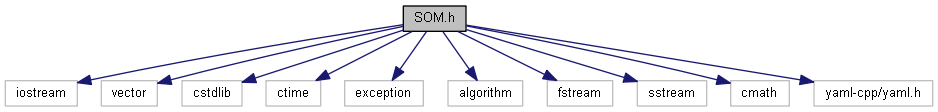
\includegraphics[width=350pt]{_s_o_m_8h__incl}
\end{center}
\end{figure}
\subsection*{Classes}
\begin{DoxyCompactItemize}
\item 
class \mbox{\hyperlink{class_s_o_m}{S\+O\+M$<$ T $>$}}
\begin{DoxyCompactList}\small\item\em Self-\/\+Organizing Maps implementation. \end{DoxyCompactList}\end{DoxyCompactItemize}
\subsection*{Macros}
\begin{DoxyCompactItemize}
\item 
\mbox{\Hypertarget{_s_o_m_8h_a1ed28332fd5185ba2579a943e4c7ea15}\label{_s_o_m_8h_a1ed28332fd5185ba2579a943e4c7ea15}} 
\#define {\bfseries E\+N\+A\+B\+L\+E\+\_\+\+R\+O\+C\+K\+S\+DB}~0
\item 
\mbox{\Hypertarget{_s_o_m_8h_ae71449b1cc6e6250b91f539153a7a0d3}\label{_s_o_m_8h_ae71449b1cc6e6250b91f539153a7a0d3}} 
\#define {\bfseries M\+\_\+\+PI}~(3.\+14159265358979323846)
\end{DoxyCompactItemize}
\subsection*{Enumerations}
\begin{DoxyCompactItemize}
\item 
enum \mbox{\hyperlink{_s_o_m_8h_a78e44725402091318ad38c42d5c34e69}{S\+O\+M\+File\+Format}} \+: unsigned char \{ \mbox{\hyperlink{_s_o_m_8h_a78e44725402091318ad38c42d5c34e69a9463f87bbed1fcdacfb8d40e185ca2bc}{S\+O\+M\+File\+Format\+::\+Y\+A\+ML}} = 0, 
\mbox{\hyperlink{_s_o_m_8h_a78e44725402091318ad38c42d5c34e69adfdef5cd5ffa240845f810e8d389c576}{S\+O\+M\+File\+Format\+::\+R\+O\+C\+K\+S\+DB}} = 1
 \}
\begin{DoxyCompactList}\small\item\em supported file formats for \mbox{\hyperlink{class_s_o_m}{S\+OM}} \end{DoxyCompactList}\item 
enum \mbox{\hyperlink{_s_o_m_8h_a55f65662fc7b41a21c646e37b51ae9d9}{B\+M\+Dist\+Type}} \+: unsigned char \{ \mbox{\hyperlink{_s_o_m_8h_a55f65662fc7b41a21c646e37b51ae9d9af19516d11f2946f894070e92fcb56b6d}{B\+M\+Dist\+Type\+::\+Uniform}} = 0, 
\mbox{\hyperlink{_s_o_m_8h_a55f65662fc7b41a21c646e37b51ae9d9a3c17d3e1cc2c7953d493d8e5c2bfbe8c}{B\+M\+Dist\+Type\+::\+Exp\+Decay}} = 1, 
\mbox{\hyperlink{_s_o_m_8h_a55f65662fc7b41a21c646e37b51ae9d9afedf7ba6075fb5526a7ace0b9385528d}{B\+M\+Dist\+Type\+::\+Gaussian}} = 2
 \}
\begin{DoxyCompactList}\small\item\em Distribution types for B\+MU neighborhood update coefficients. \end{DoxyCompactList}\item 
enum \mbox{\hyperlink{_s_o_m_8h_a69503914f8053c00b814b3096e784d72}{Distance\+Type}} \+: unsigned char \{ \mbox{\hyperlink{_s_o_m_8h_a69503914f8053c00b814b3096e784d72a3e43207685247008d9e1ae53ecf8cab3}{Distance\+Type\+::\+Euclidean}} = 0, 
\mbox{\hyperlink{_s_o_m_8h_a69503914f8053c00b814b3096e784d72a9e463ed1966bd2867f9e1c972c0c0e2f}{Distance\+Type\+::\+Dot\+Product}} = 1, 
\mbox{\hyperlink{_s_o_m_8h_a69503914f8053c00b814b3096e784d72aab1326fd2c841260ef94363765655de0}{Distance\+Type\+::\+Cosine\+Simiarity}} = 2, 
\mbox{\hyperlink{_s_o_m_8h_a69503914f8053c00b814b3096e784d72ae7179381b417596fbab1d2e5ebd90207}{Distance\+Type\+::\+Squared\+Euclidean}} = 3
 \}
\begin{DoxyCompactList}\small\item\em Distance metrics \end{DoxyCompactList}\end{DoxyCompactItemize}


\subsection{Enumeration Type Documentation}
\mbox{\Hypertarget{_s_o_m_8h_a55f65662fc7b41a21c646e37b51ae9d9}\label{_s_o_m_8h_a55f65662fc7b41a21c646e37b51ae9d9}} 
\index{S\+O\+M.\+h@{S\+O\+M.\+h}!B\+M\+Dist\+Type@{B\+M\+Dist\+Type}}
\index{B\+M\+Dist\+Type@{B\+M\+Dist\+Type}!S\+O\+M.\+h@{S\+O\+M.\+h}}
\subsubsection{\texorpdfstring{B\+M\+Dist\+Type}{BMDistType}}
{\footnotesize\ttfamily enum \mbox{\hyperlink{_s_o_m_8h_a55f65662fc7b41a21c646e37b51ae9d9}{B\+M\+Dist\+Type}} \+: unsigned char\hspace{0.3cm}{\ttfamily [strong]}}



Distribution types for B\+MU neighborhood update coefficients. 

\begin{DoxyEnumFields}{Enumerator}
\raisebox{\heightof{T}}[0pt][0pt]{\index{Uniform@{Uniform}!S\+O\+M.\+h@{S\+O\+M.\+h}}\index{S\+O\+M.\+h@{S\+O\+M.\+h}!Uniform@{Uniform}}}\mbox{\Hypertarget{_s_o_m_8h_a55f65662fc7b41a21c646e37b51ae9d9af19516d11f2946f894070e92fcb56b6d}\label{_s_o_m_8h_a55f65662fc7b41a21c646e37b51ae9d9af19516d11f2946f894070e92fcb56b6d}} 
Uniform&Same coeffs for B\+MU and all of its neighborhoods. \\
\hline

\raisebox{\heightof{T}}[0pt][0pt]{\index{Exp\+Decay@{Exp\+Decay}!S\+O\+M.\+h@{S\+O\+M.\+h}}\index{S\+O\+M.\+h@{S\+O\+M.\+h}!Exp\+Decay@{Exp\+Decay}}}\mbox{\Hypertarget{_s_o_m_8h_a55f65662fc7b41a21c646e37b51ae9d9a3c17d3e1cc2c7953d493d8e5c2bfbe8c}\label{_s_o_m_8h_a55f65662fc7b41a21c646e37b51ae9d9a3c17d3e1cc2c7953d493d8e5c2bfbe8c}} 
Exp\+Decay&exponential decay \\
\hline

\raisebox{\heightof{T}}[0pt][0pt]{\index{Gaussian@{Gaussian}!S\+O\+M.\+h@{S\+O\+M.\+h}}\index{S\+O\+M.\+h@{S\+O\+M.\+h}!Gaussian@{Gaussian}}}\mbox{\Hypertarget{_s_o_m_8h_a55f65662fc7b41a21c646e37b51ae9d9afedf7ba6075fb5526a7ace0b9385528d}\label{_s_o_m_8h_a55f65662fc7b41a21c646e37b51ae9d9afedf7ba6075fb5526a7ace0b9385528d}} 
Gaussian&Gaussian distribution \\
\hline

\end{DoxyEnumFields}
\mbox{\Hypertarget{_s_o_m_8h_a69503914f8053c00b814b3096e784d72}\label{_s_o_m_8h_a69503914f8053c00b814b3096e784d72}} 
\index{S\+O\+M.\+h@{S\+O\+M.\+h}!Distance\+Type@{Distance\+Type}}
\index{Distance\+Type@{Distance\+Type}!S\+O\+M.\+h@{S\+O\+M.\+h}}
\subsubsection{\texorpdfstring{Distance\+Type}{DistanceType}}
{\footnotesize\ttfamily enum \mbox{\hyperlink{_s_o_m_8h_a69503914f8053c00b814b3096e784d72}{Distance\+Type}} \+: unsigned char\hspace{0.3cm}{\ttfamily [strong]}}



Distance metrics 

\begin{DoxyEnumFields}{Enumerator}
\raisebox{\heightof{T}}[0pt][0pt]{\index{Euclidean@{Euclidean}!S\+O\+M.\+h@{S\+O\+M.\+h}}\index{S\+O\+M.\+h@{S\+O\+M.\+h}!Euclidean@{Euclidean}}}\mbox{\Hypertarget{_s_o_m_8h_a69503914f8053c00b814b3096e784d72a3e43207685247008d9e1ae53ecf8cab3}\label{_s_o_m_8h_a69503914f8053c00b814b3096e784d72a3e43207685247008d9e1ae53ecf8cab3}} 
Euclidean&Euclidean distance\+: For 2D, the distance between $ (x_1,y_1) $ and $ (x_2,y_2) $ is $ \sqrt{ (x_2 - x_1)^2 + (y_2 - y_1)^2 } $ . General form ( $L^2$ norm) for the vectors $A,B$ with the size $n$ is calculated as\+:

\[ \sqrt{\sum\limits_{i=1}^n (A_i - B_i)^2} \] \\
\hline

\raisebox{\heightof{T}}[0pt][0pt]{\index{Dot\+Product@{Dot\+Product}!S\+O\+M.\+h@{S\+O\+M.\+h}}\index{S\+O\+M.\+h@{S\+O\+M.\+h}!Dot\+Product@{Dot\+Product}}}\mbox{\Hypertarget{_s_o_m_8h_a69503914f8053c00b814b3096e784d72a9e463ed1966bd2867f9e1c972c0c0e2f}\label{_s_o_m_8h_a69503914f8053c00b814b3096e784d72a9e463ed1966bd2867f9e1c972c0c0e2f}} 
Dot\+Product&Dot Product\+: General form for the vectors $A,B$ with a size $n$\+:

\[ \sum\limits_{i=1}^n (A_i * B_i) \] \\
\hline

\raisebox{\heightof{T}}[0pt][0pt]{\index{Cosine\+Simiarity@{Cosine\+Simiarity}!S\+O\+M.\+h@{S\+O\+M.\+h}}\index{S\+O\+M.\+h@{S\+O\+M.\+h}!Cosine\+Simiarity@{Cosine\+Simiarity}}}\mbox{\Hypertarget{_s_o_m_8h_a69503914f8053c00b814b3096e784d72aab1326fd2c841260ef94363765655de0}\label{_s_o_m_8h_a69503914f8053c00b814b3096e784d72aab1326fd2c841260ef94363765655de0}} 
Cosine\+Simiarity&Cosine Simiarity\+: General form for the vectors $A,B$ with a size $n$ \+:

\[ \text{similarity}= \cos(\theta )={\mathbf{A} \cdot \mathbf{B} \over \|\mathbf{A} \|\|\mathbf{B} \|}= { \frac {\sum \limits _{i=1}^{n}{A_{i}B_{i} } } { \sqrt {\sum \limits _{i=1}^{n}{A_{i}^{2} } } \sqrt {\sum \limits _{i=1}^{n}{B_{i}^{2} } } } } \] \\
\hline

\raisebox{\heightof{T}}[0pt][0pt]{\index{Squared\+Euclidean@{Squared\+Euclidean}!S\+O\+M.\+h@{S\+O\+M.\+h}}\index{S\+O\+M.\+h@{S\+O\+M.\+h}!Squared\+Euclidean@{Squared\+Euclidean}}}\mbox{\Hypertarget{_s_o_m_8h_a69503914f8053c00b814b3096e784d72ae7179381b417596fbab1d2e5ebd90207}\label{_s_o_m_8h_a69503914f8053c00b814b3096e784d72ae7179381b417596fbab1d2e5ebd90207}} 
Squared\+Euclidean&Squared Euclidean\+: For 2D, the distance between $(x_1,y_1)$ and $(x_2,y_2)$ is $ (x_2 - x_1) ^ 2 + (y_2 - y_1) ^ 2 $. General form for the vectors $A,B$ with a size $n$ is calculated as\+:

\[ \sum\limits_{i=1}^n (A_i - B_i)^2 \] \\
\hline

\end{DoxyEnumFields}
\mbox{\Hypertarget{_s_o_m_8h_a78e44725402091318ad38c42d5c34e69}\label{_s_o_m_8h_a78e44725402091318ad38c42d5c34e69}} 
\index{S\+O\+M.\+h@{S\+O\+M.\+h}!S\+O\+M\+File\+Format@{S\+O\+M\+File\+Format}}
\index{S\+O\+M\+File\+Format@{S\+O\+M\+File\+Format}!S\+O\+M.\+h@{S\+O\+M.\+h}}
\subsubsection{\texorpdfstring{S\+O\+M\+File\+Format}{SOMFileFormat}}
{\footnotesize\ttfamily enum \mbox{\hyperlink{_s_o_m_8h_a78e44725402091318ad38c42d5c34e69}{S\+O\+M\+File\+Format}} \+: unsigned char\hspace{0.3cm}{\ttfamily [strong]}}



supported file formats for \mbox{\hyperlink{class_s_o_m}{S\+OM}} 

\begin{DoxyEnumFields}{Enumerator}
\raisebox{\heightof{T}}[0pt][0pt]{\index{Y\+A\+ML@{Y\+A\+ML}!S\+O\+M.\+h@{S\+O\+M.\+h}}\index{S\+O\+M.\+h@{S\+O\+M.\+h}!Y\+A\+ML@{Y\+A\+ML}}}\mbox{\Hypertarget{_s_o_m_8h_a78e44725402091318ad38c42d5c34e69a9463f87bbed1fcdacfb8d40e185ca2bc}\label{_s_o_m_8h_a78e44725402091318ad38c42d5c34e69a9463f87bbed1fcdacfb8d40e185ca2bc}} 
Y\+A\+ML&yaml file format \\
\hline

\raisebox{\heightof{T}}[0pt][0pt]{\index{R\+O\+C\+K\+S\+DB@{R\+O\+C\+K\+S\+DB}!S\+O\+M.\+h@{S\+O\+M.\+h}}\index{S\+O\+M.\+h@{S\+O\+M.\+h}!R\+O\+C\+K\+S\+DB@{R\+O\+C\+K\+S\+DB}}}\mbox{\Hypertarget{_s_o_m_8h_a78e44725402091318ad38c42d5c34e69adfdef5cd5ffa240845f810e8d389c576}\label{_s_o_m_8h_a78e44725402091318ad38c42d5c34e69adfdef5cd5ffa240845f810e8d389c576}} 
R\+O\+C\+K\+S\+DB&Rocks\+DB DB format. \\
\hline

\end{DoxyEnumFields}

%--- End generated contents ---

% Index
\backmatter
\newpage
\phantomsection
\clearemptydoublepage
\addcontentsline{toc}{chapter}{Index}
\printindex

\end{document}
